% =============================================================================
% Consolidated Phase 1-3 Report -- STRUCTURAL SKELETON ONLY
%
% This file gives you section/subsection scaffolding, figure/table placeholders
% with correct paths, and a page budget so the whole thing fits in 10 pages.
%
% IMPORTANT (per the assignment's AI-plagiarism policy on the report):
%   - Every block marked "TODO (write yourself)" is analysis/discussion/
%     reflection that must be written by YOU, in your own words. You must be
%     able to defend every sentence of it at the viva.
%   - Factual tables/numbers pulled directly from your own committed report
%     files (report/phase*_*.md) are pre-filled below as a convenience --
%     double-check every number against the source .md file before submitting,
%     since these are exactly the kind of detail you'll be asked about live.
%   - Delete this whole comment block before submitting.
%
% Compiling:
%   Local:    pdflatex final_report.tex   (run twice for refs/ToC if you add any)
%   No LaTeX installed locally? Upload this .tex + the report/figures/ folder
%   to a new Overleaf project (overleaf.com) and compile there.
%
% Page budget target (10pt font, ~2cm margins, single column):
%   Intro/setup........... ~0.5 page
%   Phase 1 (data/tok)..... ~1.5 pages
%   Phase 2 (arch/pretrain) ~3.0 pages
%   Phase 3 (finetune/attn) ~3.5 pages
%   Reflections + repro.... ~1.0 page
%   Cut figures/tables first if you overshoot -- not text.
% =============================================================================

\documentclass[10pt]{article}
\usepackage[margin=2cm]{geometry}
\usepackage{graphicx}
\usepackage{booktabs}
\usepackage{caption}
\usepackage{subcaption}
\usepackage{amsmath}
\usepackage{hyperref}
\usepackage{times}
\usepackage[table]{xcolor}

\setlength{\parskip}{0.4em}
\setlength{\parindent}{0pt}

\title{\vspace{-1.5em}Hindi and Nepali Small-LLM: Phases 1--3 Report}
\author{TODO: your name, roll number}
\date{\today}

\begin{document}
\maketitle
\vspace{-2em}

% -----------------------------------------------------------------------------
\section{Introduction}
% TODO (write yourself): 2-4 sentences. What is the overall project (build and
% evaluate small transformer LMs for Hindi and Nepali, low- vs higher-resource
% comparison), and what does each phase contribute (data -> pretraining ->
% reasoning finetuning + analysis). Point to report/phase1_summary.md,
% phase2_*.md, phase3_*.md for the detailed per-phase writeups this report
% consolidates.

% =============================================================================
\section{Phase 1: Data Collection, Cleaning, and Tokenization}
% Source detail: report/phase1_*.md (cleaning, collection, statistics,
% provenance, tokenizer, validation, manual-data, reproducibility)

\subsection{Corpora}
% TODO (write yourself): where the Hindi/Nepali corpora came from, size before/
% after cleaning, how the two languages differ in available volume (this is
% the "higher- vs lower-resource" framing that Phases 2-3 build on).

\begin{figure}[h]
  \centering
  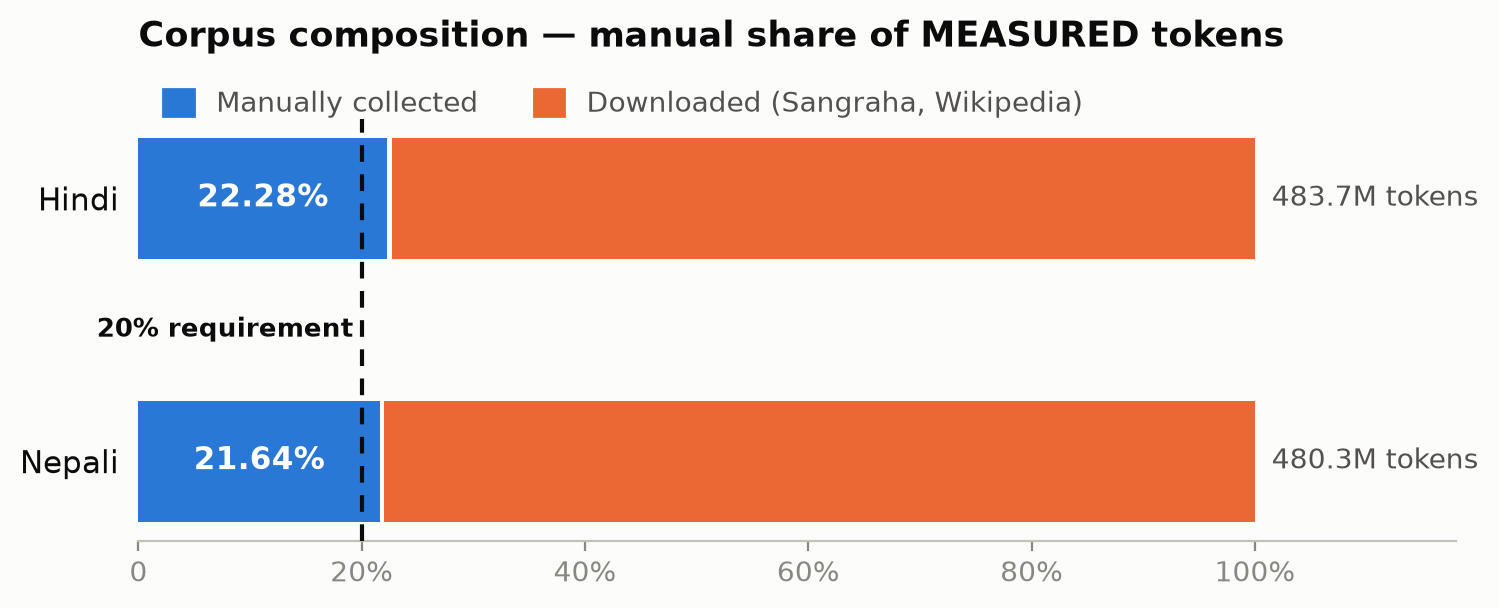
\includegraphics[width=0.48\textwidth]{figures/corpus_composition.png}
  \hfill
  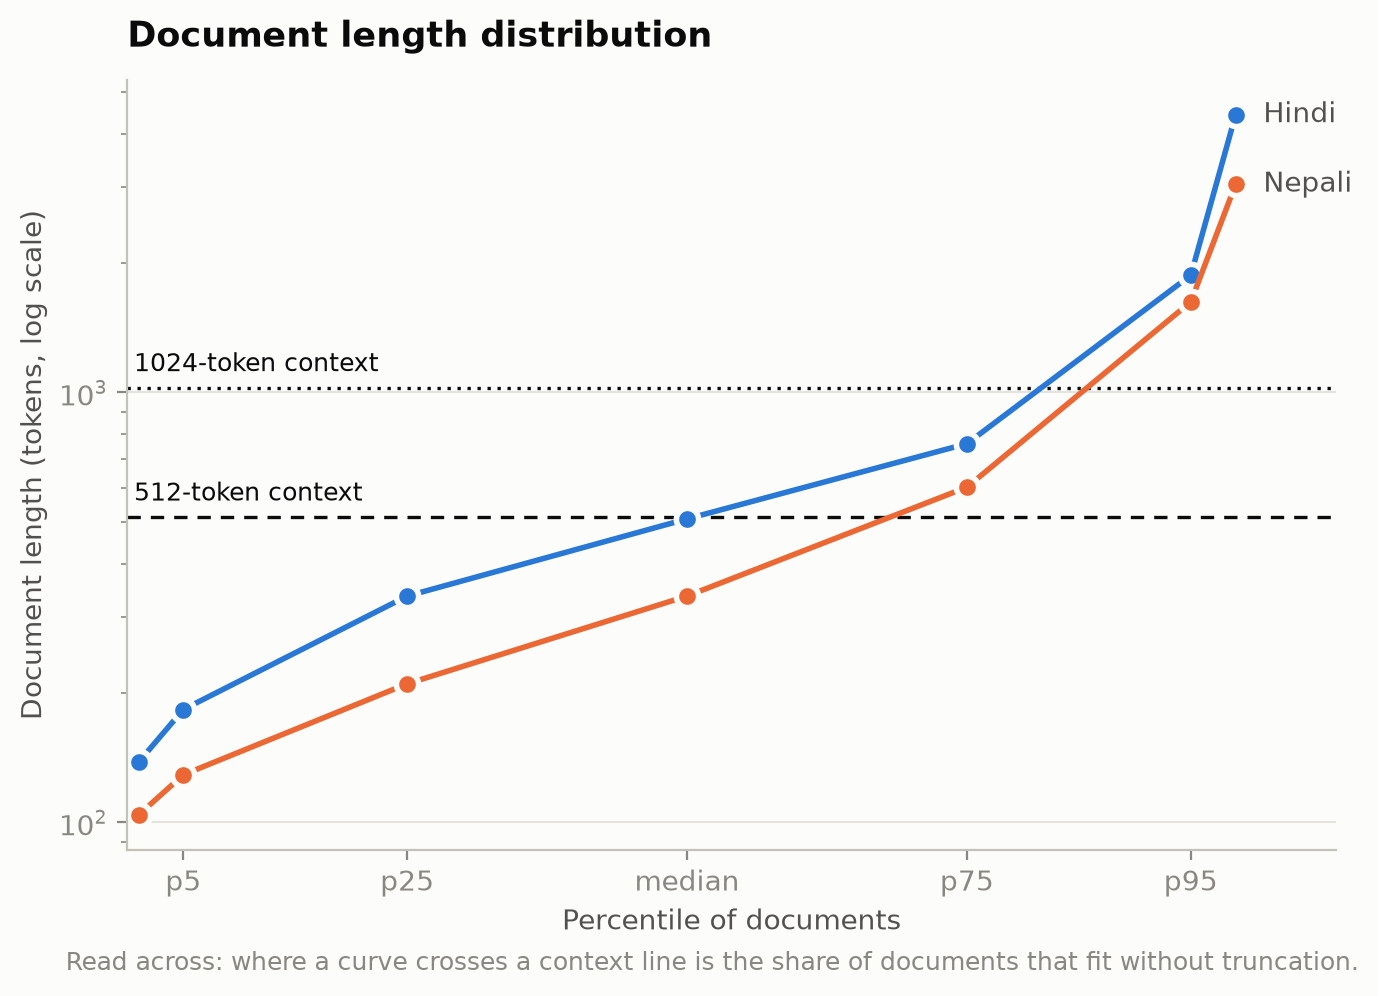
\includegraphics[width=0.48\textwidth]{figures/doc_length.png}
  \caption{Corpus composition and document-length distribution. TODO: one-line
  takeaway in your own words.}
\end{figure}

\subsection{Cleaning pipeline}
% TODO (write yourself): key cleaning/filtering steps and what they removed.
\begin{figure}[h]
  \centering
  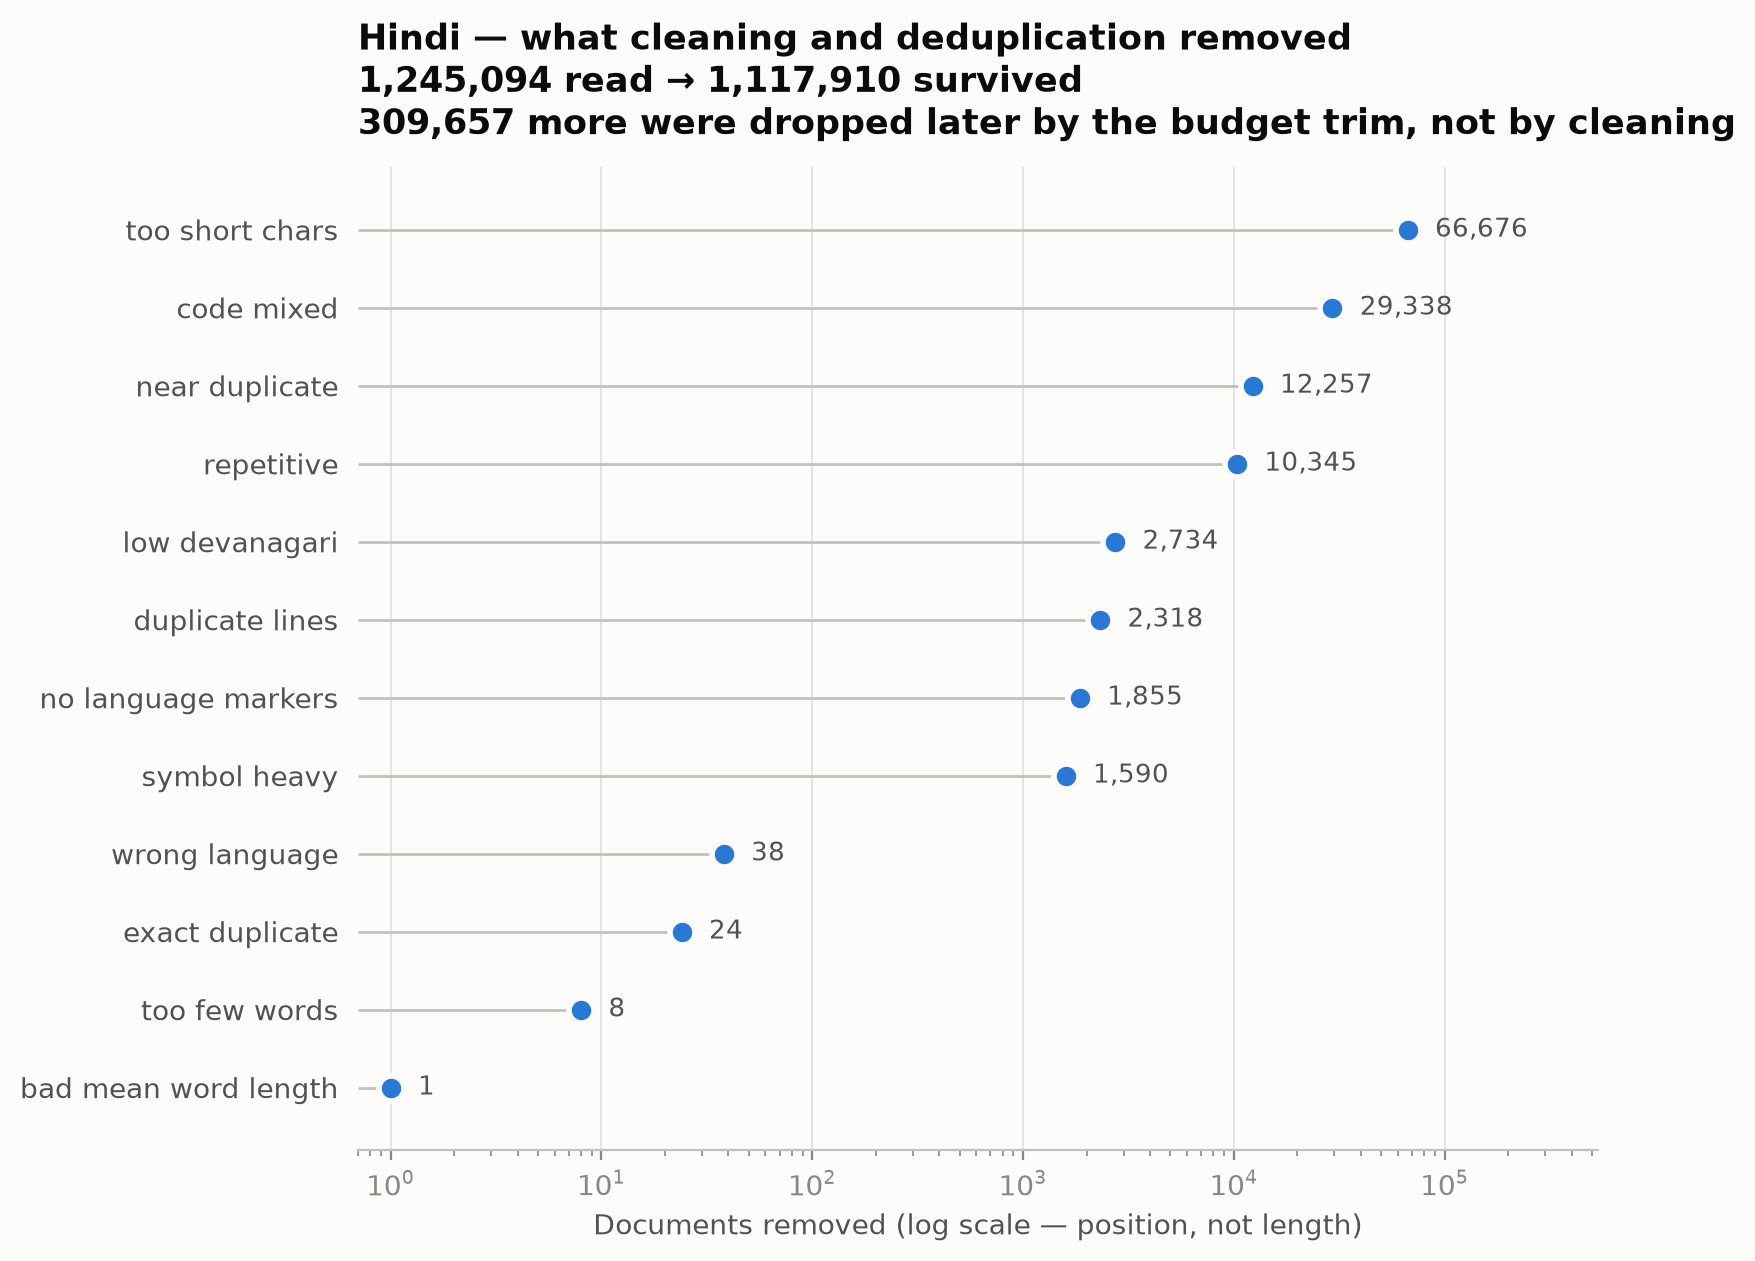
\includegraphics[width=0.6\textwidth]{figures/cleaning_hindi.png}
  \caption{Hindi cleaning pipeline effect. TODO: caption in your own words.}
\end{figure}

\subsection{Tokenizer}
% TODO (write yourself): SentencePiece choice, vocab size(s) tried, and the
% headline vocab-size finding (see report/phase2_architecture_report.md
% "Vocabulary and embedding cost" and the Phase 3 vocab-ablation result below
% in Section 4 -- cross-reference rather than duplicate).
\begin{figure}[h]
  \centering
  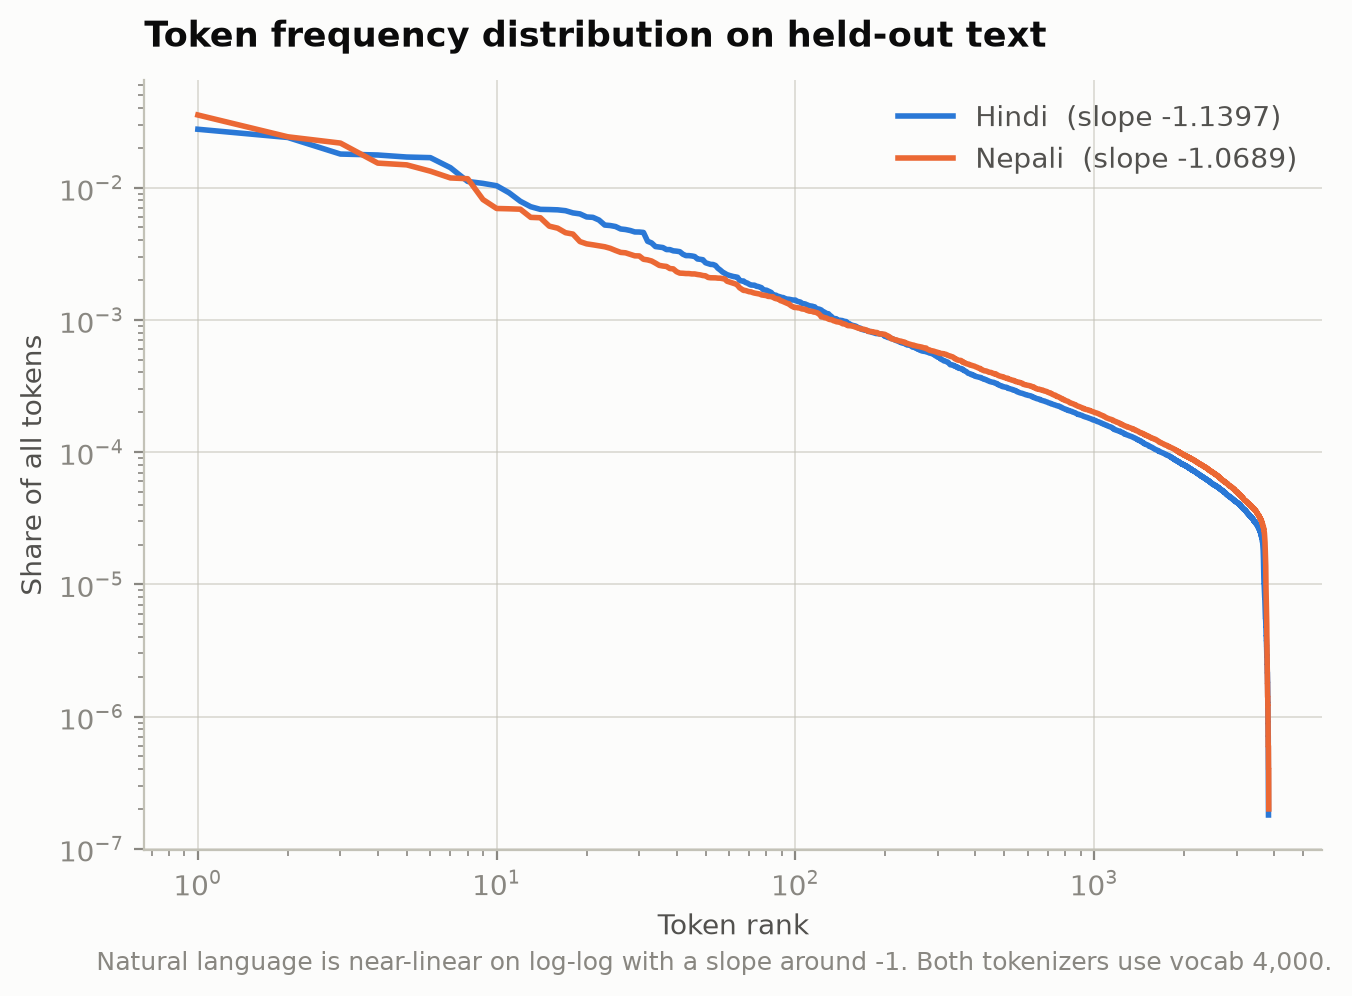
\includegraphics[width=0.55\textwidth]{figures/zipf.png}
  \caption{Token-frequency (Zipf) distribution. TODO: caption in your own words.}
\end{figure}

% =============================================================================
\section{Phase 2: Model Architecture and Pretraining}
% Source detail: report/phase2_architecture_report.md, phase2_training_report.md,
% phase2_ablation_report.md, phase2_attention_report.md, phase2_lm_evaluation_report.md

\subsection{Architecture}
% TODO (write yourself): decoder-only transformer, d_model/n_layer/n_head,
% positional embeddings, why these dims for Model H (Hindi) vs Model L (Nepali).
% Fill the table below from report/phase2_architecture_report.md.
\begin{table}[h]
\centering
\caption{Model configuration (fill exact values from phase2\_architecture\_report.md)}
\begin{tabular}{lrrrrr}
\toprule
Model & d\_model & n\_layer & n\_head & vocab & total params \\
\midrule
H (Hindi)  & TODO & TODO & TODO & TODO & TODO \\
L (Nepali) & TODO & TODO & TODO & TODO & TODO \\
\bottomrule
\end{tabular}
\end{table}

\subsection{Pretraining}
% TODO (write yourself): schedule, compute, final train/val perplexity for
% each model, and the resource-tier framing (Model H higher-resource vs
% Model L lower-resource -- how that shows up in the loss curves).
\begin{figure}[h]
  \centering
  \begin{subfigure}{0.48\textwidth}
    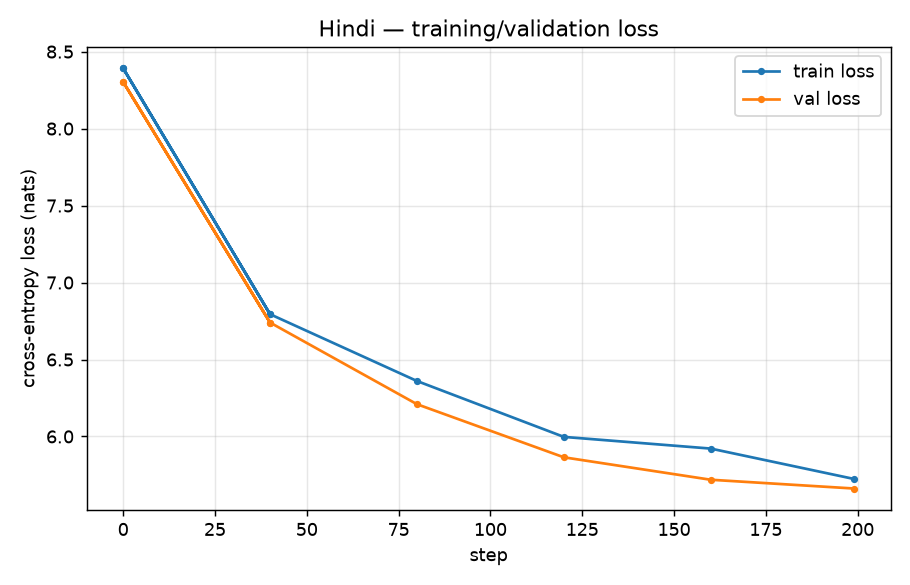
\includegraphics[width=\textwidth]{figures/phase2/hindi/loss_curve.png}
    \caption{Hindi (Model H)}
  \end{subfigure}
  \hfill
  \begin{subfigure}{0.48\textwidth}
    
\includegraphics[width=\textwidth]{figures/phase2/nepali/loss_curve.png}
    \caption{Nepali (Model L)}
  \end{subfigure}
  \caption{Pretraining loss curves. TODO: caption in your own words.}
\end{figure}

\subsection{Vocabulary-size ablation}
% Factual table -- verified in this session's full 156,250-step Phase 3
% finetuning runs across all 4 (lang x vocab) combinations. Cross-check
% against your own logs before submitting.
\begin{table}[h]
\centering
\caption{Reasoning accuracy by vocabulary size (best checkpoint vs.\ final step)}
\begin{tabular}{lrrrr}
\toprule
 & Hindi 4k & Hindi 8k & Nepali 4k & Nepali 8k \\
\midrule
Best (step 1{,}000)      & 5.00\% & 5.00\% & 10.93\% & 10.85\% \\
Final (step 156{,}250)   & 3.42\% & 3.35\% & 0\%     & 0\% \\
\bottomrule
\end{tabular}
\end{table}
% TODO (write yourself): interpretation -- vocab size (4k vs 8k) has no
% meaningful effect on either pretraining perplexity or downstream reasoning
% accuracy at this architecture/data scale; explain WHY you think that is,
% using your own reasoning about embedding-parameter share, not just the
% number. This is exactly the kind of claim you'll be asked to defend at viva.

\subsection{Positional-embedding ablation}
% TODO (write yourself): summarize the no-pos-embedding ablation result from
% report/phase2_ablation_report.md (what broke, why, and what it demonstrates
% about the architecture's reliance on position information).

% =============================================================================
\section{Phase 3: Reasoning Finetuning and Analysis}
% Source detail: report/phase3_reasoning_report.md, phase3_attention_report.md,
% phase3_final_report.md

\subsection{Synthetic reasoning dataset}
% TODO (write yourself): the nine question families, dataset size (5M
% examples/language), leakage-avoidance mechanisms, and why you chose a
% template-generated (not full-LLM-generated) dataset -- reference your own
% verification that a full-LLM-generation approach had an unacceptable
% ~37-38% wrong-answer rate on self-consistency checks, if that's relevant to
% your narrative.

\subsection{Finetuning protocol}
% TODO (write yourself): frozen-backbone regularization, why it was needed
% (near-instant overfitting without it), and the checkpoint-selection
% methodology finding -- val-loss-selected best.pt vs. measured task accuracy
% diverge sharply at this dataset scale; both landed at step 1,000 in your
% final runs, and accuracy collapses to 0\% (Nepali) well before the full
% 156,250-step schedule finishes. Explain what this implies about the
% mismatch between step budget and dataset scale.

\subsection{Pretrained vs.\ finetuned: reasoning accuracy}
% TODO (write yourself): pull the per-family accuracy table from
% report/phase3_reasoning_report.md Section 4 and discuss Model H vs Model L.

\subsection{Attention analysis: pretrained vs.\ finetuned}
% TODO (write yourself): entropy/attention-distance shift, and what the
% heatmaps show (or don't) about local vs long-range attention reorganization.
\begin{figure}[h]
  \centering
  \begin{subfigure}{0.24\textwidth}
    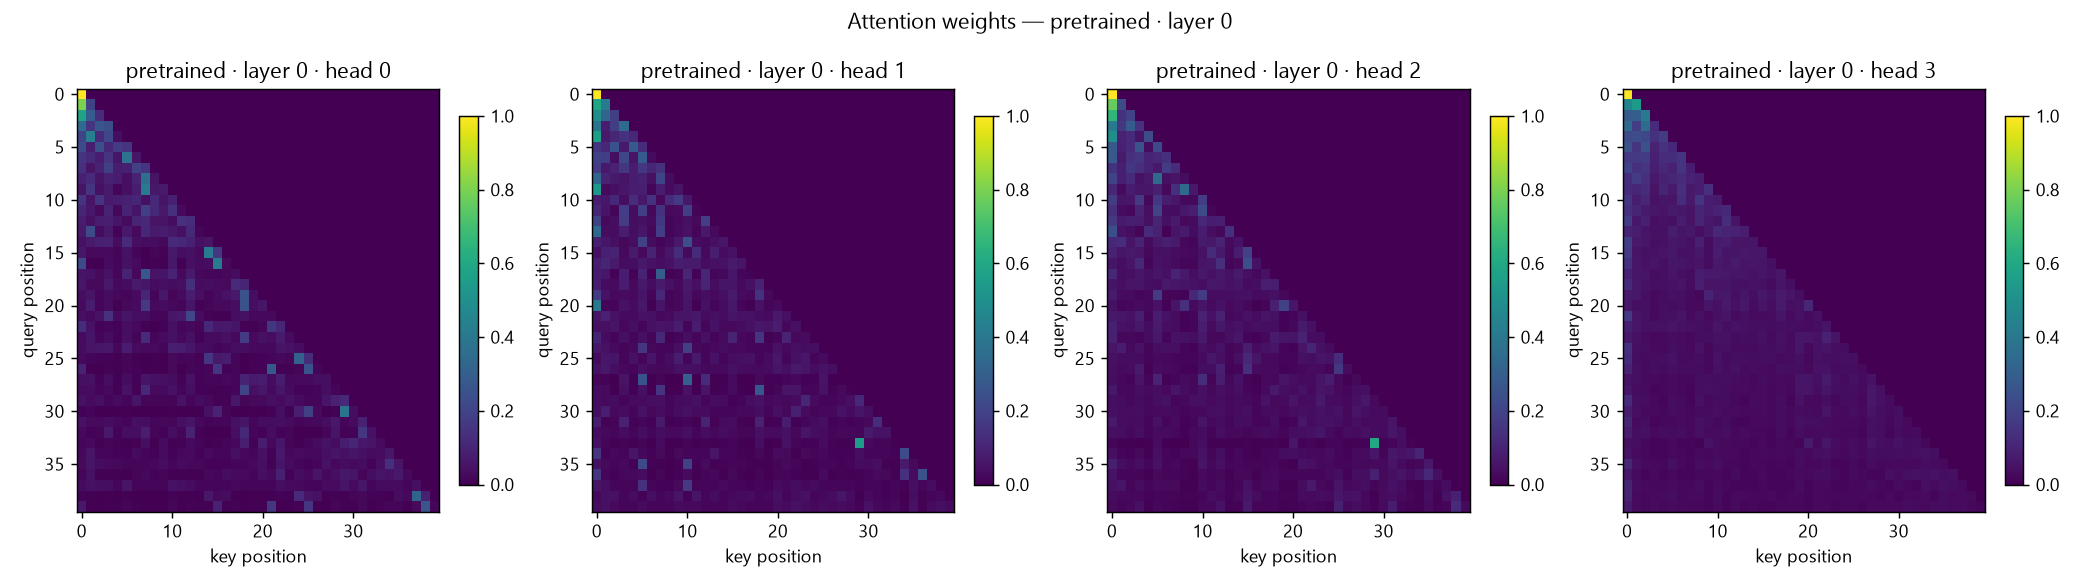
\includegraphics[width=\textwidth]{figures/phase3/hindi/attention_pretrained_vs_finetuned/pretrained_heatmap_layer_00.png}
    \caption{Pretrained, layer 0}
  \end{subfigure}
  \begin{subfigure}{0.24\textwidth}
    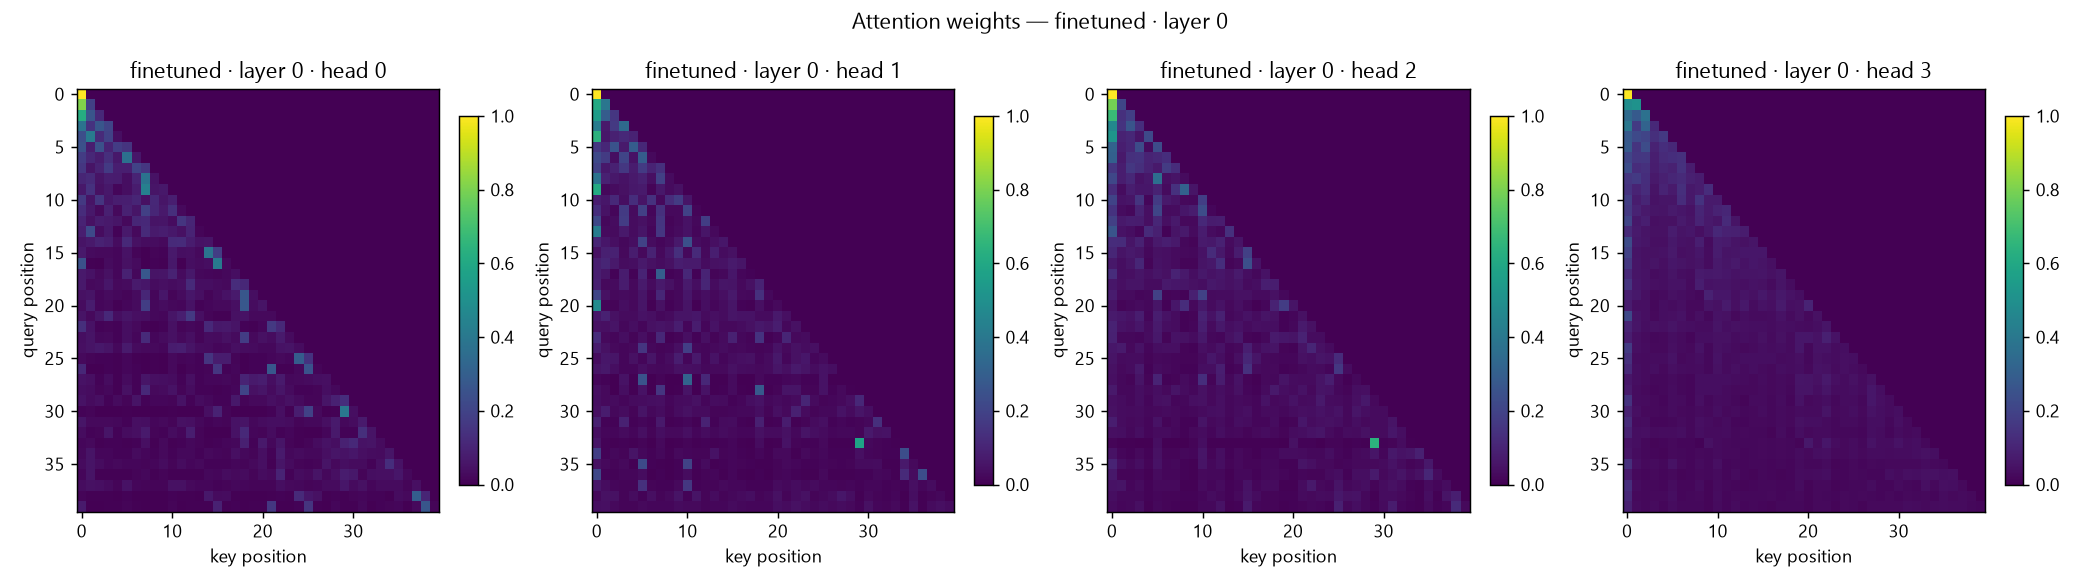
\includegraphics[width=\textwidth]{figures/phase3/hindi/attention_pretrained_vs_finetuned/finetuned_heatmap_layer_00.png}
    \caption{Finetuned, layer 0}
  \end{subfigure}
  \begin{subfigure}{0.24\textwidth}
    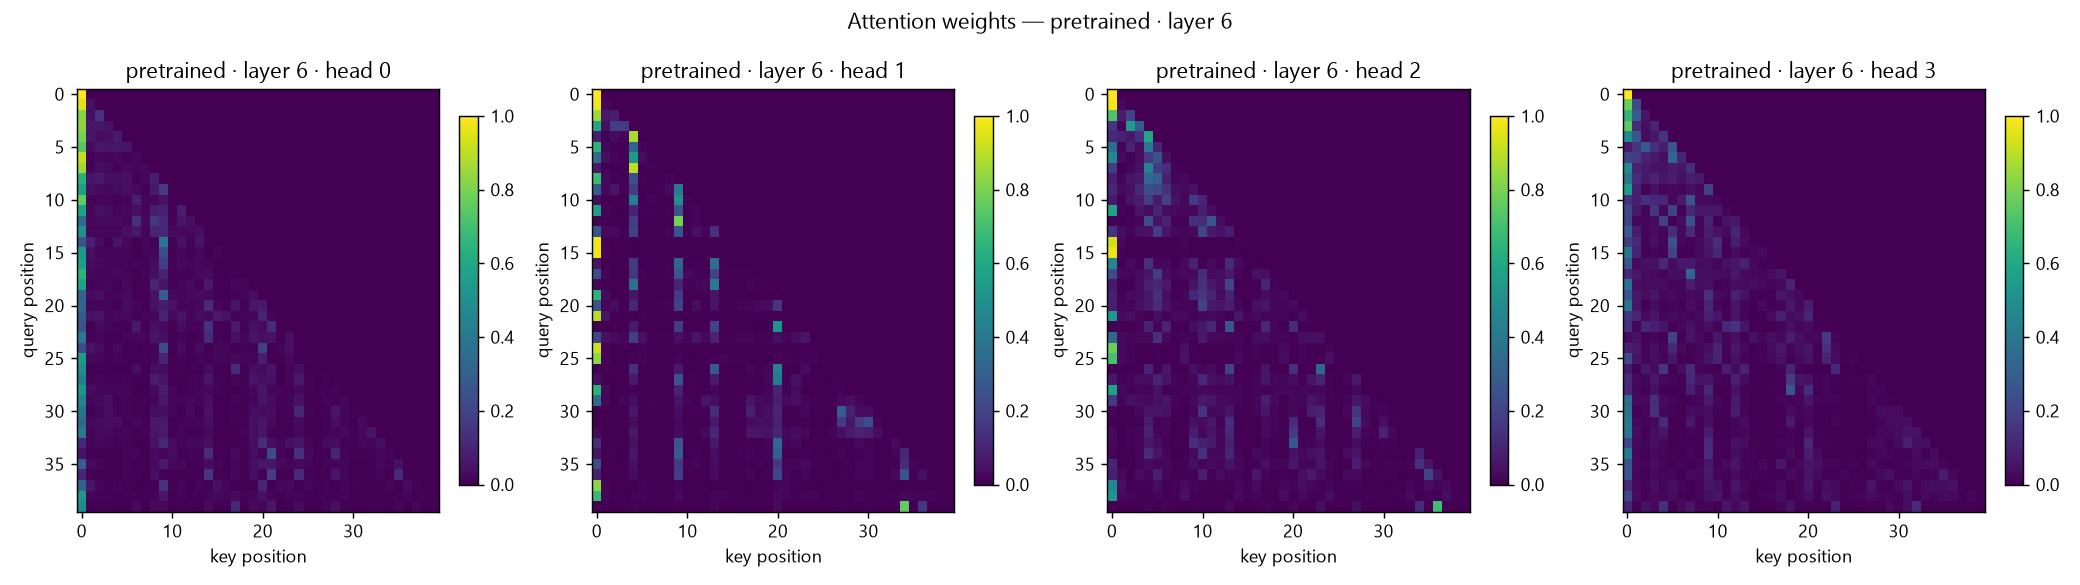
\includegraphics[width=\textwidth]{figures/phase3/hindi/attention_pretrained_vs_finetuned/pretrained_heatmap_layer_06.png}
    \caption{Pretrained, layer 6}
  \end{subfigure}
  \begin{subfigure}{0.24\textwidth}
    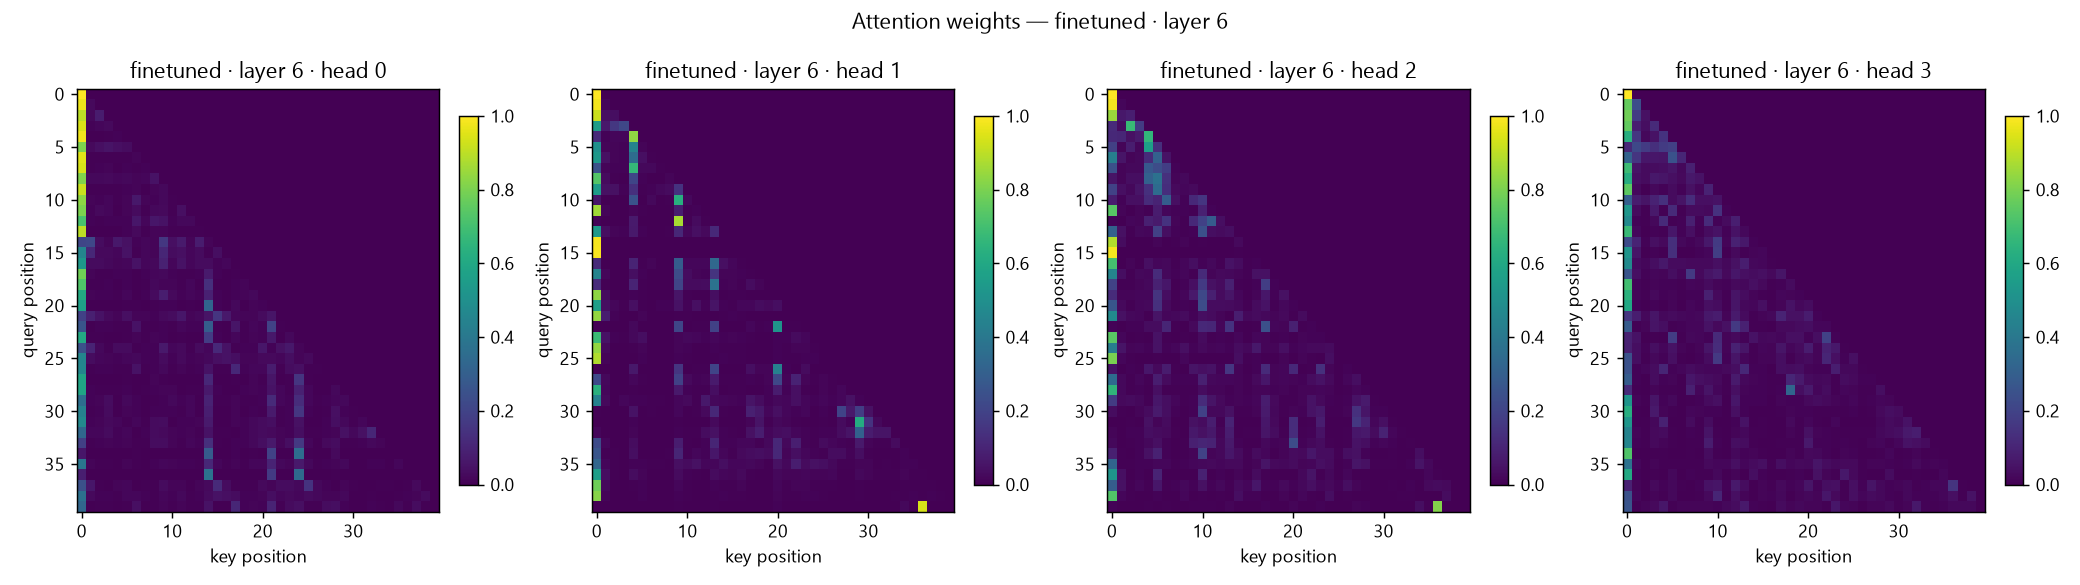
\includegraphics[width=\textwidth]{figures/phase3/hindi/attention_pretrained_vs_finetuned/finetuned_heatmap_layer_06.png}
    \caption{Finetuned, layer 6}
  \end{subfigure}
  \caption{Hindi attention heatmaps, layer 0 vs.\ layer 6 (of 7), pretrained
  vs.\ finetuned. TODO: caption/discussion in your own words. (Swap in the
  \texttt{nepali} figures too, or replace with a single representative pair
  if space is tight -- all 7 layers for both languages and both checkpoints
  are in \texttt{report/phase3\_attention\_report.md} \S4, not reproduced
  here since 28 heatmaps would blow the 10-page budget.)}
\end{figure}

\subsection{Model H vs.\ Model L: overall comparison}
% TODO (write yourself): pull the master comparison table from
% report/phase3_final_report.md Section 1 and summarize the higher- vs
% lower-resource story across all three phases in a few sentences.

% =============================================================================
\section{Reflections and Limitations}
% TODO (write yourself, entirely -- this section is exactly what the viva and
% plagiarism check will probe hardest): what would you do differently, what
% surprised you, what's the biggest limitation of the current setup (e.g.
% the finetuning step-budget/dataset-scale mismatch found in Phase 3), and
% what's still unresolved (e.g. any known bugs you chose not to fix given
% time constraints -- be honest, this is safer than hiding it).

% =============================================================================
\section{Reproducibility and Artifacts}
% TODO: verify these Drive links are current and public before submitting.
% See README.md and report/phase2_checkpoint_links.json for the canonical list.
\begin{itemize}
  \item Code: this repository, branch \texttt{phase-3}.
  \item Pretrained checkpoints (Hindi, Nepali): Google Drive links in \texttt{README.md}.
  \item Reasoning-finetuned checkpoints: TODO -- add a Drive link here if you
  are keeping a final Phase 3 checkpoint as a submission artifact (see the
  open item flagged separately: no \texttt{phase3\_checkpoint\_links.json}
  exists yet).
  \item Full per-phase detail reports: \texttt{report/phase1\_*.md},
  \texttt{report/phase2\_*.md}, \texttt{report/phase3\_*.md} in this repo.
\end{itemize}

\end{document}
